\documentclass[11pt]{article}
\usepackage[letterpaper,left=0.85in,right=1.35in,top=0.8in,bottom=0.85in]{geometry}
\usepackage{amsmath,amssymb,mathtools,booktabs,longtable,array,tabularx,xcolor,enumitem,hyperref,microtype,fancyhdr,tikz}
\usetikzlibrary{arrows.meta,positioning,shapes.geometric}
\definecolor{deepblue}{RGB}{25,64,112}
\definecolor{softblue}{RGB}{232,240,249}
\definecolor{softgreen}{RGB}{232,245,233}
\definecolor{softamber}{RGB}{255,248,225}
\definecolor{softred}{RGB}{253,235,235}
\definecolor{darkgreen}{RGB}{35,105,55}
\definecolor{darkamber}{RGB}{150,95,0}
\definecolor{darkred}{RGB}{150,35,35}
\hypersetup{colorlinks=true,linkcolor=deepblue,urlcolor=deepblue,citecolor=deepblue}
\pagestyle{fancy}
\fancyhf{}
\lhead{MP (1994): Lean Replication Architecture}
\rhead{\thepage}
\setlength{\headheight}{14pt}
\setlength{\parindent}{0pt}
\setlength{\parskip}{5pt}
\setlist[itemize]{leftmargin=1.4em,itemsep=2pt,topsep=3pt}
\setlist[enumerate]{leftmargin=1.6em,itemsep=3pt,topsep=3pt}
\newcommand{\leanhigh}{\textcolor{darkgreen}{\textbf{High-value Lean target}}}
\newcommand{\leaninfra}{\textcolor{darkamber}{\textbf{Lean-feasible, infrastructure-heavy}}}
\newcommand{\hybrid}{\textcolor{deepblue}{\textbf{Hybrid Lean + numerical target}}}
\newcommand{\outside}{\textcolor{darkred}{\textbf{Outside the core Lean target}}}
\newcommand{\papersec}[1]{\textbf{Paper location:} #1}
\newcommand{\priority}[1]{\textbf{Priority:} #1}
\newcommand{\statusbox}[2]{\colorbox{#1}{\parbox{0.94\linewidth}{#2}}}
\newcommand{\epsd}{\varepsilon_d}
\newcommand{\epsu}{\varepsilon_u}
\newcommand{\thetaM}{\vartheta}

\title{\textbf{Mortensen--Pissarides (1994)}\\
A Paper-Centered Mathematical Reconstruction and Lean 4 Replication Architecture}
\author{Prepared as a formalization contract}
\date{July 2026}

\begin{document}
\maketitle

\begin{abstract}
This document reconstructs the mathematical architecture of Mortensen and Pissarides (1994), \emph{Job Creation and Job Destruction in the Theory of Unemployment}, before any further Lean implementation. It uses the paper's notation throughout the economic exposition, separates definitions from derived claims, identifies the main theorem-level obligations, and evaluates which claims are appropriate targets for Lean 4. The principal formalization target is the analytical core of Sections 2--4 and the Appendix. Section 5 is treated as a numerical replication exercise: Lean can certify identities and selected algorithmic invariants, but simulation and calibration should be implemented in numerical software.
\end{abstract}

\statusbox{softblue}{\textbf{Guiding principle.} The project should not formalize every numbered equation as an independent theorem. The central objective is to prove a small set of economically meaningful results: the surplus and cutoff characterization, the reduced equilibrium system, existence and uniqueness, comparative statics, and the analytical claims about anticipated aggregate shocks.}

\tableofcontents
\newpage

\section{Economic setup and notation}

\subsection{Purpose and economic mechanism}
The paper embeds job-specific productivity shocks into a matching model with endogenous vacancy creation, endogenous job destruction, and bilateral surplus sharing. Existing jobs are exposed to persistent idiosyncratic shocks. Firms destroy a match only when its continuation surplus becomes non-positive. New vacancies enter until their value is zero. Aggregate productivity and the dispersion of idiosyncratic productivity jointly determine job creation, job destruction, unemployment, and vacancies.

The model's core mechanism is:
\[
\text{idiosyncratic shock} \longrightarrow \text{match surplus} \longrightarrow \text{destruction cutoff}
\]
combined with
\[
\text{free entry} \longrightarrow \text{vacancy creation} \longrightarrow \text{market tightness}.
\]
The interaction of the destruction cutoff and market tightness determines steady-state labor-market flows.

\subsection{Paper notation}
The notation below follows the paper so that each equation can be compared directly with the published text.

\begin{longtable}{>{\raggedright\arraybackslash}p{0.12\textwidth} >{\raggedright\arraybackslash}p{0.50\textwidth} >{\raggedright\arraybackslash}p{0.26\textwidth}}
\toprule
Symbol & Economic meaning & Mathematical role \\
\midrule
\endfirsthead
\toprule
Symbol & Economic meaning & Mathematical role \\
\midrule
\endhead
$p$ & Aggregate component of labor productivity or product price. & Scalar parameter. \\
$\sigma$ & Dispersion of the job-specific component; with $E[\varepsilon]=0$ and $\operatorname{Var}(\varepsilon)=1$, it is the standard deviation of $\sigma\varepsilon$. & Positive scalar parameter. \\
$\varepsilon$ & Job-specific productivity realization. & State variable. \\
$F$ & Distribution function of a fresh idiosyncratic draw. The paper assumes no mass points and finite upper support $\epsu$. & Atomless CDF / probability measure. \\
$\epsu$ & Upper support of $F$; newly created jobs begin at this productivity. & Finite scalar. \\
$\epsd$ & Endogenous reservation productivity. A job is destroyed after a draw below $\epsd$. & Endogenous cutoff. \\
$\lambda$ & Poisson arrival rate of job-specific shocks. & Positive hazard. \\
$r$ & Discount rate. & Positive scalar. \\
$c$ & Flow cost of maintaining a vacancy. & Positive scalar. \\
$b$ & Flow value of leisure or unemployment income. & Scalar. \\
$\beta$ & Worker's fixed share of match surplus. & Parameter in $(0,1)$. \\
$u$ & Unemployment, normalized by labor force. & Endogenous stock. \\
$v$ & Vacancies, normalized by labor force. & Endogenous stock. \\
$m(v,u)$ & Constant-returns matching function. & Nonnegative function, homogeneous of degree one. \\
$q(v/u)$ & Vacancy meeting rate, $m(v,u)/v=m(1,u/v)$. The paper assumes $q'<0$. & Function of market tightness. \\
$vq/u$ & Worker job-finding rate, equal to $m(v/u,1)$. & Endogenous hazard. \\
$V$ & Asset value of a vacancy. & Scalar value. \\
$J(\varepsilon)$ & Firm value of a filled job at idiosyncratic state $\varepsilon$. & Value function. \\
$W(\varepsilon)$ & Worker value of employment at $\varepsilon$. & Value function. \\
$U$ & Worker value of unemployment. & Scalar value. \\
$S(\varepsilon)$ & Total match surplus, $J(\varepsilon)+W(\varepsilon)-U$. & Surplus function. \\
$w(\varepsilon)$ & Productivity-contingent wage. & Policy / transfer. \\
\bottomrule
\end{longtable}

\subsection{Foundational assumptions}
A faithful Lean model should make the following assumptions explicit rather than leave them in prose.

\begin{enumerate}
\item \textbf{Shock distribution.} $F$ is a probability distribution on a real interval with finite upper support $\epsu$, no atoms, mean zero, and variance one. For the analytical core, mean and variance normalizations are not always needed; atomlessness and integrability matter more.
\item \textbf{Shock process.} Idiosyncratic productivity is reset at Poisson rate $\lambda$ to an independent draw from $F$.
\item \textbf{Matching technology.} $m$ is nonnegative, continuous, homogeneous of degree one, and increasing in each argument. The induced vacancy meeting rate $q(\theta)$, with $\theta=v/u$, is strictly decreasing. For uniqueness and comparative statics, one needs additional regularity, usually continuity and differentiability.
\item \textbf{Free entry.} Vacancies enter until $V=0$ whenever an interior equilibrium with positive vacancies exists.
\item \textbf{Surplus sharing.} $W(\varepsilon)-U=\beta S(\varepsilon)$ and therefore $J(\varepsilon)=(1-\beta)S(\varepsilon)$.
\item \textbf{Destruction technology.} Closing a filled job is costless, so continuation occurs precisely when $J(\varepsilon)\ge 0$.
\item \textbf{New-job productivity.} New jobs begin at $\epsu$.
\item \textbf{Interior domains.} $r>0$, $\lambda>0$, $c>0$, $0<\beta<1$, $u>0$, and $\epsd<\epsu$ for a nondegenerate equilibrium.
\end{enumerate}

\statusbox{softgreen}{\leanhigh\quad This setup is an appropriate Lean target. The main challenge is not computational but representational: the probability measure, integrals, support restrictions, and regularity of the matching function must be encoded without assuming downstream conclusions.}

\section{Steady-state model: derivation and theorem structure}

\subsection{Primitive value equations}
The paper begins with the vacancy equation and free entry:
\begin{align}
rV &= -c+q(v/u)[J(\epsu)-V], \tag{1}\\
rV &=0. \tag{2}
\end{align}
The surplus and bargaining equations are
\begin{align}
S(\varepsilon)&=J(\varepsilon)+W(\varepsilon)-U, \tag{3}\\
W(\varepsilon)-U&=\beta S(\varepsilon). \tag{4}
\end{align}
Consequently, $J(\varepsilon)=(1-\beta)S(\varepsilon)$.

For a filled job, employed worker, and unemployed worker, respectively:
\begin{align}
rJ(\varepsilon)
&=p+\sigma\varepsilon-w(\varepsilon)
+\lambda(1-\beta)\int\left\{\max[S(x),0]-S(\varepsilon)\right\}\,dF(x), \tag{5}\\
rW(\varepsilon)
&=w(\varepsilon)
+\lambda\beta\int\left\{\max[S(x),0]-S(\varepsilon)\right\}\,dF(x), \tag{6}\\
rU&=b+(vq/u)[W(\epsu)-U]. \tag{7}
\end{align}

Adding (5)--(7) and using (4) yields the central surplus equation:
\begin{equation}
(r+\lambda)S(\varepsilon)
=p+\sigma\varepsilon-b
+\lambda\int\max[S(x),0] \,dF(x)
-\beta(vq/u)S(\epsu). \tag{8}
\end{equation}

\paragraph{What is definition and what is theorem?}
Equations (1), (3), (5)--(7) define equilibrium value relationships. Free entry (2) and bargaining (4) are equilibrium restrictions. Equation (8) is the first genuine derived identity: it must be proved by algebra from (3)--(7), not placed in an assumptions structure.

\subsection{Surplus monotonicity and reservation destruction}
Because the right-hand side of (8) depends on $\varepsilon$ only through $\sigma\varepsilon$, subtraction at two states gives
\[
(r+\lambda)[S(\varepsilon_2)-S(\varepsilon_1)]
=\sigma(\varepsilon_2-\varepsilon_1).
\]
Hence, for $\sigma>0$,
\begin{equation}
S(\varepsilon_2)-S(\varepsilon_1)
=\frac{\sigma}{r+\lambda}(\varepsilon_2-\varepsilon_1). \tag{12$'$}
\end{equation}
This is stronger and more primitive than differentiating (8): it proves that $S$ is affine without initially requiring differentiability. If a cutoff $\epsd$ satisfies $S(\epsd)=0$, then
\begin{equation}
S(\varepsilon)-S(\epsd)
=\frac{\sigma(\varepsilon-\epsd)}{r+\lambda}. \tag{12}
\end{equation}
Thus $S$ is strictly increasing and destruction has a threshold form.

\subsubsection*{Core Theorem 1: Affine surplus and reservation rule}
\textbf{Statement.} Suppose $S$ satisfies (8), $r+\lambda>0$, and $\sigma>0$. Then $S$ is strictly increasing and affine with slope $\sigma/(r+\lambda)$. If there exists $\epsd$ with $S(\epsd)=0$, it is unique, $S(\varepsilon)<0$ for $\varepsilon<\epsd$, and $S(\varepsilon)>0$ for $\varepsilon>\epsd$.

\papersec{Section 3, pp. 400--402; equations (8), (9), and (12).}

\statusbox{softgreen}{\leanhigh\quad This is the best first substantive Lean theorem. It is economically central, requires only ordered-field algebra once (8) is available, avoids premature measure-theoretic differentiation, and establishes the legitimate cutoff structure needed downstream.}

\subsection{Integral representation and job-destruction condition}
Using threshold destruction, $\max[S(x),0]=S(x)$ for $x\ge \epsd$ and zero below. The paper integrates by parts to write
\begin{align}
(r+\lambda)S(\varepsilon)
&=p+\sigma\varepsilon-b
+\lambda\int_{\epsd}^{\epsu}S'(x)[1-F(x)]\,dx
-\beta(vq/u)S(\epsu) \notag\\
&=p+\sigma\varepsilon-b
+\frac{\sigma\lambda}{r+\lambda}
\int_{\epsd}^{\epsu}[1-F(x)]\,dx
-\beta(vq/u)S(\epsu). \tag{9}
\end{align}
Evaluating at $\epsd$, using $S(\epsd)=0$, and using free entry to replace $S(\epsu)$ produces the job-destruction condition
\begin{equation}
p+\sigma\epsd
=b+\frac{\beta c}{1-\beta}\frac vu
-\frac{\sigma\lambda}{r+\lambda}
\int_{\epsd}^{\epsu}[1-F(x)]\,dx. \tag{10}
\end{equation}
The three terms on the right are unemployment income, the forgone expected gain from search, and the option value of retaining a low-productivity match.

\subsubsection*{Core Theorem 2: Job-destruction equation}
\textbf{Statement.} Under the value equations, free entry, bargaining, affine surplus, a valid cutoff $\epsd$, and the required integration-by-parts conditions, the cutoff solves (10).

\papersec{Section 3, pp. 401--402; equations (9)--(10).}

\statusbox{softamber}{\leaninfra\quad The economic algebra is straightforward, but a faithful proof requires a probability measure associated with $F$, integrability of the survival function, and a rigorous tail-integral identity. A practical implementation can first prove (10) from a named tail-integral lemma, then later prove that lemma in full measure-theoretic generality.}

\subsection{Job-creation condition}
Free entry and (1)--(4) imply
\[
q(v/u)(1-\beta)S(\epsu)=c.
\]
Using (12) at $\epsu$ yields
\begin{equation}
q(v/u)=\frac{c}{1-\beta}\frac{r+\lambda}{\sigma(\epsu-\epsd)}. \tag{13}
\end{equation}
This is the job-creation condition. A higher cutoff shortens expected match surplus and therefore requires a lower market tightness, which raises the vacancy-filling rate $q$.

\subsubsection*{Core Theorem 3: Job-creation equation}
\textbf{Statement.} If free entry holds and $S$ satisfies the affine cutoff representation, then market tightness satisfies (13).

\papersec{Section 3, p. 402; equations (1)--(4), (12), and (13).}

\statusbox{softgreen}{\leanhigh\quad This is an elementary but economically important theorem. It should be proved immediately after the affine-surplus theorem.}

\subsection{Reduced steady-state equilibrium}
Let $\theta=v/u$. The analytical steady-state system consists of two equations in $(\theta,\epsd)$:
\begin{align*}
\mathrm{JD}(\theta,\epsd)&:
&&p+\sigma\epsd
=b+\frac{\beta c}{1-\beta}\theta
-\frac{\sigma\lambda}{r+\lambda}
\int_{\epsd}^{\epsu}[1-F(x)]\,dx,\\
\mathrm{JC}(\theta,\epsd)&:
&&q(\theta)=\frac{c(r+\lambda)}{(1-\beta)\sigma(\epsu-\epsd)}.
\end{align*}
The paper argues graphically that JD slopes upward in $(\epsd,\theta)$ space and JC slopes downward, giving a unique intersection.

\subsubsection*{Core Theorem 4: Equivalence between value equilibrium and reduced equilibrium}
\textbf{Statement.} Under the foundational assumptions, any value equilibrium with an interior cutoff induces a pair $(\theta,\epsd)$ satisfying (10) and (13). Conversely, a solution to (10) and (13), together with the affine surplus formula and the implied value allocations, constructs a value equilibrium.

\papersec{Section 3, pp. 400--403.}

\statusbox{softgreen}{\leanhigh\quad This bridge is more important than merely encoding equations (10) and (13). It ensures the reduced system is derived from, and is sufficient for, the original economic equilibrium. It should be a principal formalization milestone.}

\subsubsection*{Core Theorem 5: Existence and uniqueness of steady-state $(\theta,\epsd)$}
The paper states that (10) and (13) uniquely determine $v/u$ and $\epsd$. A Lean-ready theorem must specify conditions sufficient for existence as well as uniqueness. A natural route is:

\begin{itemize}
\item $q$ is continuous and strictly decreasing on an appropriate positive domain;
\item the JD equation defines a strictly increasing relation $\theta_{JD}(\epsd)$;
\item the JC equation defines a strictly decreasing relation $\theta_{JC}(\epsd)$;
\item endpoint inequalities ensure the two curves cross.
\end{itemize}

Strict opposite slopes establish at most one intersection; they do not alone establish existence. Endpoint conditions or a global range condition for $q$ are required.

\papersec{Section 3, p. 402 and Figure 1.}

\statusbox{softamber}{\leaninfra\quad This is a central theorem but requires careful theorem design. The paper's claim is informal and omits explicit endpoint conditions. The formal target should state a corrected theorem with transparent continuity and boundary assumptions.}

\subsection{Steady-state unemployment and the Beveridge relation}
Unemployment evolves according to inflows from job destruction and outflows through matching. In steady state,
\begin{equation}
u=\frac{\lambda F(\epsd)}{\lambda F(\epsd)+m(v/u,1)}. \tag{14}
\end{equation}
This follows from
\[
(1-u)\lambda F(\epsd)=u\,m(v/u,1).
\]
The paper emphasizes that the slope of the Beveridge curve in $(u,v)$ space is ambiguous because a rise in vacancies both increases matching and, through the equilibrium cutoff, may increase destruction.

\subsubsection*{Core Theorem 6: Steady-state unemployment identity}
\textbf{Statement.} If unemployment inflows and outflows are as above, flow balance is equivalent to (14).

\papersec{Section 3, pp. 403--404.}

\statusbox{softgreen}{\leanhigh\quad The flow-balance identity is easy and appropriate for Lean. The global slope or convexity of the Beveridge curve is not a theorem without additional assumptions and should not be formalized as an unconditional result.}

\section{Comparative statics: theorem catalog}

The paper mixes partial-equilibrium derivatives holding $\theta=v/u$ fixed with full-equilibrium comparative statics allowing both $\theta$ and $\epsd$ to adjust. A formal replication must keep these conceptually distinct.

\subsection{Partial-equilibrium cutoff effects}
From (10), holding $\theta$ fixed:

\begin{enumerate}
\item A rise in $p-b$ lowers $\epsd$.
\item A rise in the expected search return $\frac{\beta c}{1-\beta}\theta$ raises $\epsd$.
\item A rise in $\lambda$ lowers $\epsd$ because faster redrawing raises the option value of waiting.
\item A rise in $r$ raises $\epsd$ because future recovery is discounted more heavily.
\item The effect of $\sigma$ on $\epsd$ depends on the profitability of the marginal job. The paper's equation (11) states
\begin{equation}
\sigma\frac{\partial\epsd}{\partial\sigma}
=\frac{r+\lambda}{r+\lambda F(\epsd)}
\left(p-b-\frac{\beta c}{1-\beta}\theta\right). \tag{11}
\end{equation}
\end{enumerate}

\subsubsection*{Theorem 7: Partial comparative statics of the destruction cutoff}
\papersec{Section 3, pp. 401--402; equations (10)--(11).}

\statusbox{softamber}{\leaninfra\quad These are valuable Lean targets, but the implementation should avoid invoking informal ``differentiation'' unless differentiability has been established. For $p$ and $b$, monotone comparative statics can often be proved directly from strict monotonicity. For $\lambda$, $r$, and $\sigma$, derivative identities require calculus and the fundamental theorem for parameterized integrals.}

\subsection{Full-equilibrium steady-state comparative statics}
Combining JD and JC, the paper and Appendix establish:

\begin{center}
\begin{tabularx}{0.96\textwidth}{@{}lXX@{}}
\toprule
Parameter change & Market tightness $\theta=v/u$ & Cutoff $\epsd$ \\
\midrule
$p$ increases & increases & decreases \\
$b$ increases & decreases & increases \\
$\lambda$ increases & decreases & decreases \\
$r$ increases & decreases & ambiguous \\
$\sigma$ increases & increases & generally increases under a sufficient condition such as $p\ge b$ \\
\bottomrule
\end{tabularx}
\end{center}

The Appendix differentiates the two-equation system. It proves $\partial\theta/\partial\lambda<0$, $\partial\theta/\partial r<0$, and $\partial\theta/\partial\sigma>0$, while the sign of $\partial\epsd/\partial r$ remains ambiguous. A sufficient condition for $\partial\epsd/\partial\sigma>0$ is $p\ge b$.

\subsubsection*{Core Theorem 8: Equilibrium comparative statics}
\textbf{Statement.} Under differentiability, nondegeneracy of the Jacobian, and the paper's matching-elasticity restrictions, the reduced equilibrium responds to $(p,b,\lambda,r,\sigma)$ with the signs summarized above.

\papersec{Section 3, pp. 402--404; Appendix, pp. 413--414, equations (A1)--(A12).}

\statusbox{softamber}{\leaninfra\quad This is one of the paper's most important theorem families. It is suitable for Lean, but only after the reduced equilibrium and uniqueness theorem are in place. A robust approach is to formalize a two-equation implicit-function comparative-statics lemma and then instantiate it.}

\subsection{Flow implications}
Conditional on current unemployment $u$:

\begin{itemize}
\item A positive aggregate productivity shock raises job creation and lowers job destruction.
\item A rise in dispersion raises both job creation and job destruction.
\item A rise in $\lambda$ lowers job creation; its effect on destruction is potentially offset by the endogenous fall in $\epsd$.
\end{itemize}

These flow claims are derived from the comparative statics of $\theta$ and $\epsd$ together with
\[
\text{creation}=m(v,u)=vq(\theta),
\qquad
\text{destruction}=\lambda F(\epsd)(1-u).
\]

\subsubsection*{Core Theorem 9: Sign of creation and destruction responses}
\papersec{Section 3, p. 404.}

\statusbox{softgreen}{\leanhigh\quad Once equilibrium comparative statics are available, these are short corollaries. They should not be treated as independent assumptions.}

\section{Cyclical shocks and dynamic analytical results}

\subsection{Two-state aggregate productivity}
Section 4 allows $p$ to jump between a low value $p$ and a high value $p^*>p$ at Poisson rate $\mu$. Market tightness and the cutoff are forward-looking jump variables; unemployment evolves continuously except for the discrete destruction of newly unprofitable matches when the economy enters recession.

The unemployment law of motion for a fixed aggregate state is
\begin{equation}
\dot u=(1-u)\lambda F(\epsd)-u\,m(v/u,1). \tag{15}
\end{equation}
The coupled surplus equations are (16)--(18), distinguishing low-state jobs, high-state jobs that survive a downturn, and high-state jobs that would be destroyed in a downturn.

\subsection{Reservation cutoffs under anticipated transitions}
The paper derives boom and recession cutoff equations (20) and (24). Their economic content is:

\begin{itemize}
\item Anticipating a future downturn reduces the option value of marginal jobs in the boom and raises the boom cutoff relative to the corresponding isolated steady state.
\item Anticipating a future recovery raises the option value of marginal jobs in recession and lowers the recession cutoff relative to the isolated recession steady state.
\item Therefore, anticipation narrows the gap between boom and recession cutoffs.
\end{itemize}

\subsubsection*{Extension Theorem 10: Anticipation compresses cutoff cyclicality}
\papersec{Section 4, pp. 405--407; equations (16)--(24).}

\statusbox{softamber}{\leaninfra\quad This is a meaningful Lean target. The two-state system is finite-dimensional, but the proof still uses piecewise surplus functions and tail integrals. It should follow only after the steady-state infrastructure is complete.}

\subsection{Job creation with anticipated transitions}
The paper derives a recession job-creation condition similar to (13), equation (28), and a modified boom condition, equation (30). It concludes that
\[
(v/u)^*>v/u,
\]
so job creation is higher in the boom, but anticipated switching reduces the boom creation rate relative to a comparison of isolated steady states.

\subsubsection*{Extension Theorem 11: Boom creation exceeds recession creation, but anticipation dampens creation cyclicality}
\papersec{Section 4, p. 407; equations (25)--(30).}

\statusbox{softamber}{\leaninfra\quad Suitable for Lean after the two-state surplus system has been constructed. The ``dampens cyclicality'' statement must be formalized relative to a clear benchmark, typically the $\mu=0$ counterfactual with fixed cutoffs or the fully recomputed isolated steady states.}

\subsection{Asymmetric job-destruction dynamics}
When $p$ falls from $p^*$ to $p$, all jobs with idiosyncratic states between the new and old cutoffs are destroyed immediately. There is no symmetric instantaneous employment increase in a boom because new matches require search. The paper argues that this asymmetry makes job destruction more volatile and causes destruction to lead creation in recessions.

\subsubsection*{Extension Theorem 12: Impact asymmetry at aggregate-state transitions}
A Lean-ready statement should distinguish three claims:

\begin{enumerate}
\item If the recession cutoff exceeds the boom cutoff, the transition into recession destroys the mass of existing matches in the interval between them.
\item A transition into boom has no corresponding instantaneous creation because matching is a flow process.
\item Under a specified employment distribution, the recession impact destruction is nonnegative and strictly positive when that interval has positive mass.
\end{enumerate}

\papersec{Section 4, pp. 407--408.}

\statusbox{softgreen}{\leanhigh\quad The qualitative impact asymmetry is an excellent Lean target once an employment measure is defined. The stronger claim that destruction is quantitatively ``more volatile'' is not a pure theorem without a stochastic process, metric, and distributional assumptions.}

\subsection{Dispersion shocks}
When $\sigma$ switches between high and low states, the paper concludes that job creation and job destruction move in the same direction. It states inequality (31) to show that the direct effect of dispersion on creation dominates the indirect effect through the cutoff.

\subsubsection*{Extension Theorem 13: Dispersion shocks generate positive comovement}
\papersec{Section 4, pp. 408--409; equation (31).}

\statusbox{softamber}{\leaninfra\quad This is a legitimate analytical target, but the paper sketches rather than fully derives the result. A formal version must state the conditions under which inequality (31) holds and distinguish impact from steady-state responses.}

\section{General Markov equilibrium and employment dynamics}

Before simulation, the paper states the equilibrium conditions for a general Markov process for aggregate productivity $p$. Let $G(dp'\mid p)$ denote the transition kernel. The equilibrium is summarized by a state-contingent meeting rate and cutoff, with surplus $S(\varepsilon,p)$. The relevant system is given by equations (32)--(34), followed by the law of motion of the employment distribution and flow accounting in equations (35)--(38).

\subsection{General Markov equilibrium characterization}
The core analytical obligation is not numerical solution; it is to state precisely what constitutes a Markov equilibrium and show that the finite-state two-state system is a specialization.

\subsubsection*{Extension Theorem 14: General Markov equilibrium contains the steady-state and two-state models as special cases}
\papersec{Section 5, pp. 409--410; equations (32)--(34).}

\statusbox{softamber}{\leaninfra\quad This is feasible but foundational. A general measurable-state Markov kernel requires substantial probability infrastructure. A finite aggregate-state formalization is more proportionate for the first project and still captures the paper's simulation environment.}

\subsection{Employment-distribution law of motion}
Let $n_t(\varepsilon)$ denote the distribution of existing jobs across idiosyncratic states. Equation (35) updates the distribution after idiosyncratic redraws, aggregate transitions, cutoff destruction, and creation at $\epsu$. Equations (36)--(38) define creation, destruction, and the employment accounting identity
\begin{equation}
N_{t+1}=N_t+C_t-D_t. \tag{38}
\end{equation}

\subsubsection*{Extension Theorem 15: Mass accounting and preservation}
\textbf{Statement.} Given a well-defined transition operator and flow definitions, the next-period employment measure is nonnegative, has the claimed total mass, and satisfies the accounting identity (38).

\papersec{Section 5, pp. 409--410; equations (35)--(38).}

\statusbox{softgreen}{\leanhigh\quad This is a good formal target. Lean is well suited to verify measure nonnegativity, mass decomposition, and accounting identities. It is less well suited to replace the numerical computation of the equilibrium policy functions.}

\section{Simulation and calibration: appropriate scope}

Section 5 discretizes aggregate productivity into a three-state Markov chain, assumes a uniform idiosyncratic distribution, chooses a log-linear matching function, calibrates parameters, solves equations (32)--(34), simulates 100 samples, and compares simulated job-flow moments with U.S. manufacturing data.

\subsection{What Lean should verify}
\begin{itemize}
\item The transition matrix is stochastic: entries are nonnegative and rows sum to one.
\item The uniform distribution and matching-function specialization satisfy the stated assumptions.
\item Given computed policy vectors, the equilibrium residuals are within a certified tolerance, if rational or interval arithmetic is used.
\item The employment update preserves mass and satisfies (38).
\item Definitions of creation and destruction rates are internally consistent.
\end{itemize}

\subsection{What should be done in numerical software}
\begin{itemize}
\item Solve the nonlinear Markov equilibrium system.
\item Generate Monte Carlo realizations.
\item Compute simulated standard deviations and correlations.
\item Match moments and compare with the data.
\item Reproduce tables and figures.
\end{itemize}

\statusbox{softred}{\outside\quad Requiring Lean to reproduce Monte Carlo estimates or calibration is not a good use of the theorem prover. These are numerical and statistical exercises, not deductive proofs. A hybrid workflow should use Python or Julia for computation and Lean only for certified structural properties or exact residual checks.}

\section{Prioritized Lean roadmap}

\subsection{What are the key theorems of the paper?}
The paper does not present formally numbered propositions. Its theorem-level contribution is distributed across equations and prose. The following ranked list converts the paper into a manageable formal proof program.

\begin{longtable}{>{\raggedright\arraybackslash}p{0.06\textwidth} >{\raggedright\arraybackslash}p{0.25\textwidth} >{\raggedright\arraybackslash}p{0.17\textwidth} >{\raggedright\arraybackslash}p{0.36\textwidth}}
\toprule
Rank & Theorem family & Paper section & Why it matters / Lean priority \\
\midrule
\endfirsthead
\toprule
Rank & Theorem family & Paper section & Why it matters / Lean priority \\
\midrule
\endhead
1 & Affine surplus and unique destruction cutoff & Section 3, eqs. (8), (12) & Foundational economic mechanism. Establishes monotonicity and the reservation rule without circular assumptions. High-value and elementary after (8). \\
2 & Derivation of job-destruction and job-creation equations & Section 3, eqs. (9), (10), (13) & Produces the paper's reduced equilibrium system from the primitive value equations. This is the central analytical reduction. \\
3 & Equivalence of value equilibrium and reduced equilibrium & Section 3 & Prevents equations (10) and (13) from becoming detached assumptions. Essential for a faithful replication. \\
4 & Existence and uniqueness of steady-state equilibrium & Section 3, Figure 1 & The paper asserts uniqueness. Formalization must supply omitted continuity and endpoint conditions. Core theorem, moderate difficulty. \\
5 & Full-equilibrium comparative statics & Section 3 and Appendix & Delivers the paper's principal economic predictions for $p,b,\lambda,r,\sigma$. Infrastructure-heavy but central. \\
6 & Creation/destruction comovement under aggregate versus dispersion shocks & Sections 3--4 & Captures the headline result: aggregate shocks imply negative comovement; dispersion shocks imply positive comovement. \\
7 & Anticipation compresses cutoff and creation cyclicality & Section 4, eqs. (16)--(30) & Important dynamic extension. Finite-state but piecewise and integral-heavy. \\
8 & Impact asymmetry of recession versus boom & Section 4 & Explains why destruction is sharper at recession onset. Good theorem once employment distributions are formalized. \\
9 & Steady-state unemployment and flow accounting & Section 3 eq. (14); Section 5 eqs. (35)--(38) & Straightforward, reusable, and economically important, but downstream of the core equilibrium. \\
10 & General Markov equilibrium & Section 5, eqs. (32)--(34) & Conceptually broad, but expensive in generality. Prefer finite aggregate states initially. \\
11 & Simulation and calibration results & Section 5 & Numerical replication, not a core Lean target. Use Python/Julia; optionally certify identities or residual bounds. \\
\bottomrule
\end{longtable}

\subsection{Recommended milestone sequence}

\paragraph{Milestone 0: New formalization contract and clean primitives.}
Create a new branch or directory while retaining the old project as an archive. Implement only paper primitives, probability objects, matching assumptions, and value-equilibrium equations. Do not include cutoff uniqueness, monotonicity, reduced equilibrium, or comparative statics in assumption structures.

\paragraph{Milestone 1: Surplus algebra and cutoff theorem.}
\begin{itemize}
\item Derive equation (8) from (3)--(7).
\item Prove the surplus-difference identity directly.
\item Prove affine surplus, strict monotonicity, uniqueness of any zero, and the reservation destruction rule.
\item Derive equation (12) as a corollary.
\end{itemize}
\textbf{Paper location:} Section 3, equations (3)--(8), (12). \\
\textbf{Difficulty:} elementary to moderate. \\
\textbf{Why first:} it is the first genuine theorem and makes the cutoff economically legitimate.

\paragraph{Milestone 2: Reduced equilibrium equations.}
\begin{itemize}
\item Build the tail-integral lemma needed for equation (9).
\item Derive job destruction (10).
\item Derive job creation (13) from free entry and affine surplus.
\end{itemize}
\textbf{Paper location:} Section 3, equations (9)--(13). \\
\textbf{Difficulty:} moderate, driven by integration. \\
\textbf{Output:} a theorem that every value equilibrium induces a reduced equilibrium pair.

\paragraph{Milestone 3: Converse construction and equilibrium equivalence.}
Given $(\theta,\epsd)$ satisfying (10) and (13), construct $S,J,W,U,V,w$ and prove the primitive value equations. This is the most important safeguard against a merely symbolic encoding.

\paragraph{Milestone 4: Existence and uniqueness.}
State explicit boundary and regularity assumptions and prove a unique intersection of JD and JC. Keep ``at most one'' and ``exists'' as separate lemmas.

\paragraph{Milestone 5: Comparative statics.}
First prove monotone results that do not require derivatives. Then build a reusable implicit-function/Jacobian layer for the Appendix results. Derive flow implications as corollaries.

\paragraph{Milestone 6: Two-state aggregate shocks.}
Formalize a finite two-state aggregate process, piecewise surplus functions, boom/recession cutoffs, and the anticipation results. Prove impact asymmetry using an employment measure.

\paragraph{Milestone 7: Finite-state Markov employment dynamics.}
Prove transition-kernel validity, mass preservation, and flow accounting. Connect this layer to an external numerical solver.

\subsection{What should not block the core proof}
The following tasks should be postponed rather than treated as prerequisites:

\begin{itemize}
\item fully general measurable aggregate-state spaces;
\item formal Monte Carlo convergence;
\item exact reproduction of calibrated moments;
\item empirical data ingestion;
\item graphical reproduction of Figures 1 and 2;
\item proving a downward-sloping Beveridge curve without the additional dominance assumption explicitly acknowledged by the paper.
\end{itemize}

\section{Suggested Lean file architecture}

\begin{verbatim}
MP1994/
  Primitives.lean          -- parameters, F, matching technology
  Values.lean              -- V, J, W, U, S, wage, value equilibrium
  Surplus.lean             -- equation (8), affine surplus, cutoff theorem
  TailIntegral.lean        -- survival-function integration lemmas
  ReducedEquilibrium.lean  -- equations (10), (13), equivalence
  Existence.lean           -- existence and uniqueness of (theta, epsilon_d)
  ComparativeStatics.lean -- Section 3 and Appendix
  TwoState.lean            -- Section 4 aggregate shocks
  EmploymentMeasure.lean   -- distribution dynamics and flow accounting
  FiniteMarkov.lean        -- finite aggregate-state specialization
  Audit.lean               -- no-sorry and axiom checks

docs/
  mp1994_lean_architecture.tex
  mp1994_lean_architecture.pdf
  theorem_status.tex
\end{verbatim}

The old repository should be mined for reusable lemmas only after each declaration is checked against this architecture. A compiling declaration should not be migrated if it assumes the theorem it is intended to prove.

\section{Adequacy rules for the restarted project}

A result receives a green status only when all four conditions hold:

\begin{enumerate}
\item The Lean statement matches a clearly stated paper-level theorem or a transparent corrected version.
\item The conclusion is derived from primitives and named analytic lemmas, not stored in an equilibrium or assumptions record.
\item The proof has no \texttt{sorry}, no hidden axioms beyond standard classical mathematics, and no arbitrary witness that violates economic admissibility.
\item The human-readable document states the exact assumptions, proof idea, Lean declaration, and any difference from the paper.
\end{enumerate}

Amber should be used for results conditional on a named analytic closure assumption or proved only in a finite-state specialization. Red should be used for missing results, circular assumptions, or claims whose mathematical statement remains unclear.

\section{Bottom line}

The paper's proof program should be understood as a hierarchy:

\begin{center}
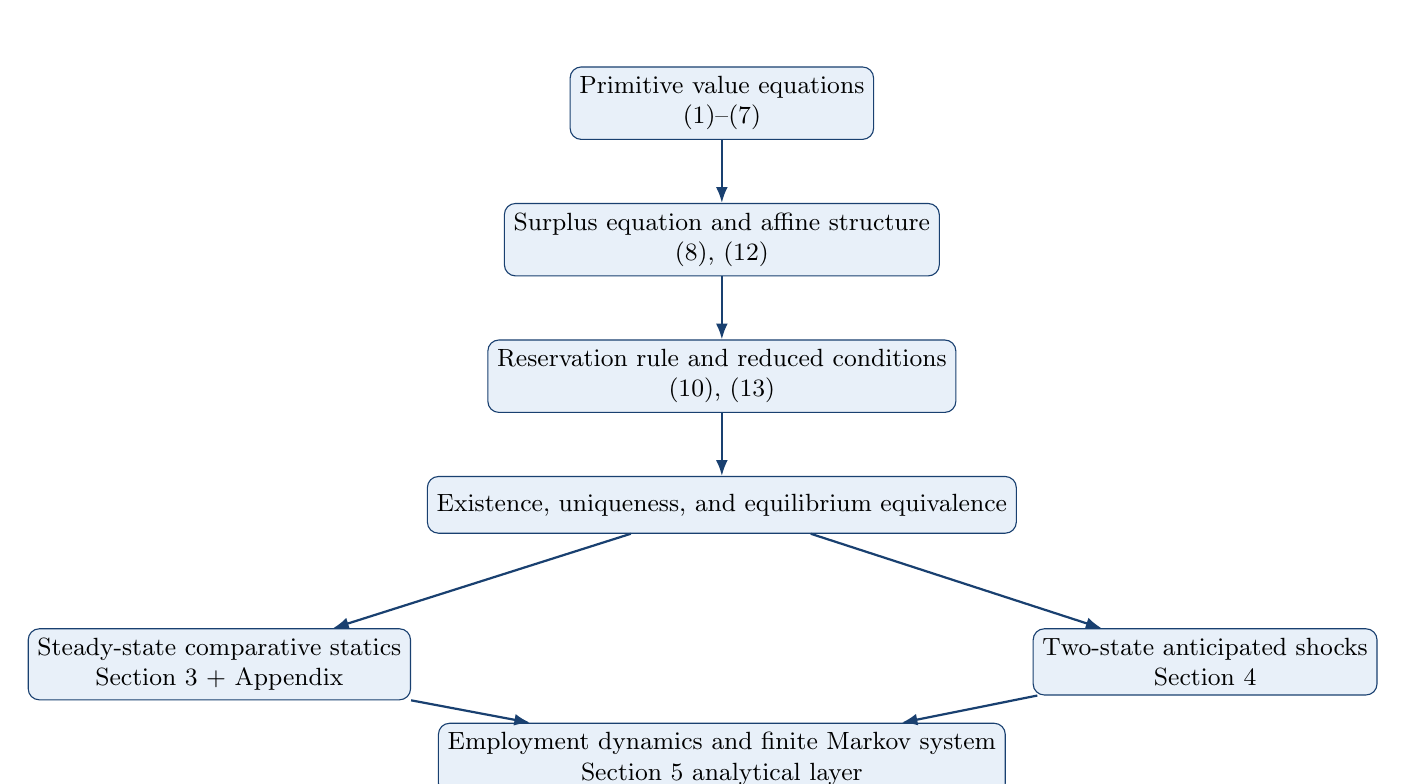
\begin{tikzpicture}[node distance=8mm and 9mm, every node/.style={font=\small,align=center}, box/.style={draw=deepblue,rounded corners,fill=softblue,minimum width=3.55cm,minimum height=0.72cm}, arr/.style={-{Latex[length=2mm]},thick,deepblue}]
\node[box] (a) {Primitive value equations\\(1)--(7)};
\node[box,below=of a] (b) {Surplus equation and affine structure\\(8), (12)};
\node[box,below=of b] (c) {Reservation rule and reduced conditions\\(10), (13)};
\node[box,below=of c] (d) {Existence, uniqueness, and equilibrium equivalence};
\node[box,below left=12mm and 2mm of d] (e) {Steady-state comparative statics\\Section 3 + Appendix};
\node[box,below right=12mm and 2mm of d] (f) {Two-state anticipated shocks\\Section 4};
\node[box,below=24mm of d] (g) {Employment dynamics and finite Markov system\\Section 5 analytical layer};
\draw[arr] (a)--(b);\draw[arr] (b)--(c);\draw[arr] (c)--(d);\draw[arr] (d)--(e);\draw[arr] (d)--(f);\draw[arr] (e)--(g);\draw[arr] (f)--(g);
\end{tikzpicture}
\end{center}

The first proof task is therefore not ``equation (12) in isolation.'' It is the first milestone: derive the surplus equation from the primitive value system, prove affine surplus and the unique reservation rule, and obtain (12) as a corollary. This places the equation inside the paper's actual economic logic and provides a reliable foundation for every subsequent result.

\end{document}
